\section{Matched simulation comparisons}\label{sec:simulation}
\subsection{Models, targets and calibration}
We evaluate eight calibrations on identical data: one-matching exact McNemar--Holm, eight-matching p-value aggregation, evidence aggregation over eight or 64 matchings, direct full-U-statistic Hoeffding--Holm, the full-sample rectangular Hoeffding comparator, Gaussian multiplier contrasts, and Gaussian multiplier edge rectangles. The rectangular methods produce orders over the same fixed family as their direct comparators, and every method passes through the same projections.

For the separated Gaussian model, $X_i=a_i Z+\sqrt{1-a_i^2}\epsilon_i$, with independent standard normals, $a_0=0.99$ and the other loadings equally spaced over $[0.45,0.55]$. The near-tie model uses $a_0=0.8+0.5/\sqrt n$, $a_1=0.8$, with other loadings in $[0.45,0.55]$. The $t_5$ model divides each Gaussian row by an independent $\sqrt{\chi_5^2/5}$. These models have a unique population star centred at zero; their population Kendall weights equal $2\arcsin(\rho)/\pi$.

Gaussian independence and IID uniform coordinates on $\{-1,0,1\}$ evaluate null comparisons and exact ties. Every labelled tree is optimal in these null models, so coverage must include degree ranges $[1,p-1]$ and rank ranges $[1,p]$, rather than the degrees of one tie-broken tree. Two additional Gaussian tree models avoid restricting the comparison to a uniquely dominant star. The chain has parent correlation $0.75$; the two-hub model has bridge correlation $0.5$ and leaf-parent correlation $0.7$, with five leaves attached to each hub at $p=12$. All population tree edges are unique optima, but equal vertex degrees retain their full tied rank ranges.

The 24 cells comprise 7,800 independent datasets. At $p=12$, the three star designs use $n\in\{252,1008,4096\}$ and 200 datasets per cell. At $p=52$, they use $n\in\{252,4096\}$ and 100 per cell. Gaussian null cells at $p=12$ use all three sizes, and at $p=52$ use $n=1008$; the discrete null uses $p=12,n=1008$. Every null cell has 1,000 datasets. Chain and two-hub cells use $p=12,n\in\{1008,4096\}$ and 100 datasets per cell. All tests use $\alpha=0.05$, and multiplier calibration uses 999 draws. Seeds, complete cell definitions and individual outcomes are archived.

We report false-order FWER, simultaneous degree and rank coverage, interval widths, forced edges, possible hubs and unique-hub declarations. Wilson intervals quantify Monte Carlo uncertainty. With 1,000 repetitions, the Monte Carlo standard error at probability $0.05$ is about $0.007$. A single empirical rejection proportion is not interpreted as a proof or disproof of a coverage theorem.

\subsection{Test, projection and family ablations}
For every test we compare marginal rank projection, direct degree-difference projection, degree conservation, and their intersection, using the same screened minor. This isolates computational changes from statistical calibration. For the first 100 datasets in every $p=12$ cell, we also add the cycle-path LP and optimize all ordered degree differences, rather than only anchor differences. Improvements are checked independently with Python arbitrary-precision integers. Empty order relations and a forced single tree have known sharp endpoints, so redundant LP solves are skipped. Path-stage estimates therefore have 100 repetitions per cell and are compared with the corresponding paired subset of the other stages.

The complete-edge comparison family is evaluated on the same first 100 non-null datasets in each $p=12$ cell. All four $p=12$ null cells extend both families to 1,000 datasets. Comparisons of families use matched subsets; differences in reported means do not arise from different simulated samples.

\subsection{A frequency reference from practice}
Bootstrap edge reliability is widely used in correlation networks \citep{tumminello2007,musciotto2018}. On the same $p=12$ separated-star, near-tie and Gaussian-null samples with $n=1008$ and $4096$, we compute 499 ordinary Pearson row-bootstrap trees. Pearson and Kendall have the same population optimal-tree ordering in these Gaussian designs. We record edge selection frequencies and the frequency with which the observed anchor is the unique highest-degree vertex. A threshold of $0.95$ is evaluated as a practical declaration rule, including its false hub and false forced-edge rates. It is a frequency heuristic, not a simultaneous confidence procedure. This reference uses all 200 non-null and all 1,000 null datasets in the six selected cells.

\subsection{Calibration and power results}
Table~\ref{tab:nullnew} reports null FWER for the common minor-plus-joint-rank projection. Exact methods have their finite-sample guarantee; the multiplier methods are evaluated empirically. All cellwise Wilson intervals, simultaneous coverage outcomes and replication records accompany the article.
\begin{table}[htbp]\centering\small
\setlength{\tabcolsep}{4pt}
\caption{False-order FWER at nominal 0.05; 1,000 datasets in each null cell. P: one-matching exact; M8: merged p-values; E8/E64: evidence aggregation over 8/64 matchings; M-C: multiplier contrasts; M-B: multiplier rectangle. Both Hoeffding controls have zero false orders in these cells. All methods use the local family.}\label{tab:nullnew}
\begin{lrbox}{\resultsbox}\begin{tabular}{lrrrrrr}
\toprule
Model, $p$, $n$ & P & M8 & E8 & E64 & M-C & M-B\\
\midrule
Gaussian null, 12, 252 & 0.024 & 0.000 & 0.000 & 0.001 & 0.072 & 0.002\\
Gaussian null, 12, 1008 & 0.029 & 0.000 & 0.000 & 0.000 & 0.062 & 0.003\\
Gaussian null, 12, 4096 & 0.032 & 0.000 & 0.001 & 0.000 & 0.042 & 0.001\\
Discrete null, 12, 1008 & 0.029 & 0.000 & 0.001 & 0.000 & 0.050 & 0.001\\
Gaussian null, 52, 1008 & 0.035 & 0.000 & 0.000 & 0.000 & 0.077 & 0.000\\
\bottomrule\end{tabular}\end{lrbox}\ifdim\wd\resultsbox>\linewidth\resizebox{\linewidth}{!}{\usebox{\resultsbox}}\else\usebox{\resultsbox}\fi\end{table}
The largest one-matching null estimate is 0.035, with an individual Wilson interval [0.025,0.048] (Gaussian null, $p=52$, $n=1008$). This is a cellwise Monte Carlo summary; simultaneous calibration is established by the exact-test argument.
\begin{table}[htbp]\centering\small
\setlength{\tabcolsep}{4pt}
\caption{Probability of declaring the true unique hub using the same minor and joint-rank projection. Local comparisons; 200 repetitions for the displayed $p=12$ star cells and 100 for $p=52$. Both Hoeffding controls declare no unique hub in these star cells; full results are archived. Path projection is evaluated separately on paired subsets.}\label{tab:powernew}
\begin{lrbox}{\resultsbox}\begin{tabular}{lrrrrrr}
\toprule
Model, $p$, $n$ & P & M8 & E8 & E64 & M-C & M-B\\
\midrule
Gaussian star, 12, 1008 & 0.000 & 0.000 & 0.000 & 0.000 & 1.000 & 0.900\\
Gaussian star, 12, 4096 & 1.000 & 0.990 & 1.000 & 1.000 & 1.000 & 1.000\\
$t_5$ star, 12, 1008 & 0.000 & 0.000 & 0.000 & 0.000 & 1.000 & 0.195\\
$t_5$ star, 12, 4096 & 1.000 & 1.000 & 1.000 & 1.000 & 1.000 & 1.000\\
Gaussian star, 52, 4096 & 0.670 & 0.000 & 1.000 & 1.000 & 1.000 & 1.000\\
$t_5$ star, 52, 4096 & 0.720 & 0.000 & 1.000 & 1.000 & 1.000 & 1.000\\
Near-tie star, 12, 4096 & 0.000 & 0.000 & 0.000 & 0.000 & 0.000 & 0.000\\
Near-tie star, 52, 4096 & 0.000 & 0.000 & 0.000 & 0.000 & 0.000 & 0.000\\
\bottomrule\end{tabular}\end{lrbox}\ifdim\wd\resultsbox>\linewidth\resizebox{\linewidth}{!}{\usebox{\resultsbox}}\else\usebox{\resultsbox}\fi\end{table}
Power is interpreted jointly with FWER. The multiplier contrast procedure exceeds nominal error in some IID null cells; higher declaration rates in those regimes do not establish valid superiority. The exact evidence methods provide a comparison whose error guarantee does not rely on the Gaussian approximation.
Figure~\ref{fig:powernew} compares the full sample-size grids. The merged rule is assessed as an exact alternative, rather than assumed to recover U-statistic efficiency. The bounded-range U-statistic comparator shows whether using all pairs alone is sufficient; the matched multiplier rectangle and contrast procedures isolate the effect of shared-edge covariance and direct calibration.
\begin{figure}[htbp]\centering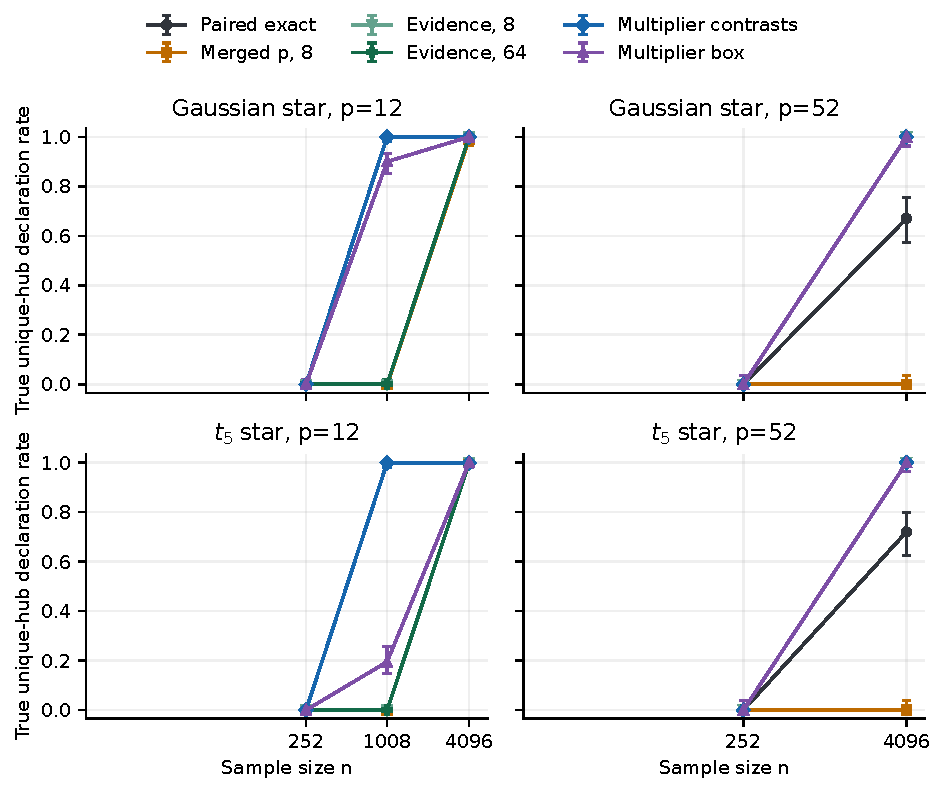
\includegraphics[width=\textwidth]{Fig_comparative.pdf}
\caption{Unique-hub declarations under the common joint projection. Curves use matched data; intervals are individual 95\% Wilson Monte Carlo intervals. All specified sample sizes and both separated distributions are shown.}\label{fig:powernew}\end{figure}
\subsection{Projection ablation}
\begin{table}[htbp]\centering\small
\setlength{\tabcolsep}{4pt}
\caption{Paired projection ablation at $p=12,n=1008$, using the same first 100 datasets per cell. Degree widths compare the minor with path LP. Rank widths compare marginal, joint pair/conservation and path projection. Complete results for all eight tests and sizes are archived. Width is upper minus lower endpoint.}\label{tab:ablation}
\begin{lrbox}{\resultsbox}\begin{tabular}{llrrrrr}
\toprule
Model & Test & $W_d$ minor & $W_d$ path & $W_r$ marg. & $W_r$ joint & $W_r$ path\\
\midrule
Gaussian star & P & 8.94 & 8.40 & 11.00 & 11.00 & 11.00\\
Gaussian star & E64 & 9.02 & 8.33 & 11.00 & 11.00 & 11.00\\
Gaussian star & M-C & 0.00 & 0.00 & 9.17 & 9.17 & 9.17\\
Near-tie star & P & 9.92 & 9.45 & 11.00 & 11.00 & 11.00\\
Near-tie star & E64 & 9.99 & 9.51 & 11.00 & 11.00 & 11.00\\
Near-tie star & M-C & 3.93 & 3.54 & 11.00 & 10.90 & 10.81\\
Chain & P & 8.00 & 4.58 & 11.00 & 11.00 & 11.00\\
Chain & E64 & 6.48 & 3.97 & 11.00 & 10.99 & 10.99\\
Chain & M-C & 0.00 & 0.00 & 7.67 & 7.67 & 7.67\\
Two hubs & P & 8.43 & 6.66 & 11.00 & 10.96 & 10.96\\
Two hubs & E64 & 5.82 & 5.11 & 10.98 & 10.54 & 10.54\\
Two hubs & M-C & 0.58 & 0.58 & 7.67 & 7.67 & 7.67\\
\bottomrule\end{tabular}\end{lrbox}\ifdim\wd\resultsbox>\linewidth\resizebox{\linewidth}{!}{\usebox{\resultsbox}}\else\usebox{\resultsbox}\fi\end{table}
The local-family path stage solves 950{,}820 LP objectives and independently verifies 375{,}946 improving rational certificates. The paired subsets show the contribution of path restrictions after fixing calibration. Degree-conservation and direct-pair rank results are additionally recorded as separate stages.
\subsection{Comparison-family ablation}
\begin{table}[htbp]\centering\small
\setlength{\tabcolsep}{4pt}
\caption{Matched local/complete family ablation at $p=12,n=4096$, 100 datasets per cell. Closed-order counts use the same $m(m-1)$ potential ordered pairs in either family. More tested comparisons also incur a larger multiplicity penalty.}\label{tab:family}
\begin{lrbox}{\resultsbox}\begin{tabular}{llrrrrrr}
\toprule
Model & Test & Orders L & Orders A & $W_d$ L & $W_d$ A & $W_r$ L & $W_r$ A\\
\midrule
Gaussian star & P & 113.0 & 530.7 & 0.14 & 0.25 & 9.17 & 9.17\\
Gaussian star & E64 & 110.8 & 579.0 & 0.00 & 0.00 & 9.17 & 9.17\\
Gaussian star & M-C & 214.4 & 643.0 & 0.00 & 0.00 & 9.17 & 9.17\\
$t_5$ star & P & 112.0 & 527.8 & 0.17 & 0.31 & 9.17 & 9.17\\
$t_5$ star & E64 & 110.5 & 573.7 & 0.00 & 0.00 & 9.17 & 9.17\\
$t_5$ star & M-C & 193.3 & 629.0 & 0.00 & 0.00 & 9.17 & 9.17\\
Near-tie star & P & 137.3 & 331.6 & 6.40 & 7.20 & 11.00 & 11.00\\
Near-tie star & E64 & 170.8 & 393.1 & 5.53 & 6.54 & 10.99 & 11.00\\
Near-tie star & M-C & 331.1 & 969.4 & 1.66 & 1.67 & 10.16 & 10.17\\
Chain & P & 850.2 & 1338.6 & 0.14 & 0.00 & 7.98 & 7.67\\
Chain & E64 & 923.0 & 1396.0 & 0.00 & 0.00 & 7.67 & 7.67\\
Chain & M-C & 1374.2 & 1766.2 & 0.00 & 0.00 & 7.67 & 7.67\\
Two hubs & P & 624.1 & 1117.3 & 0.99 & 0.38 & 7.67 & 7.67\\
Two hubs & E64 & 659.5 & 1157.1 & 0.97 & 0.02 & 7.67 & 7.67\\
Two hubs & M-C & 725.3 & 1538.1 & 0.00 & 0.00 & 7.67 & 7.67\\
\bottomrule\end{tabular}\end{lrbox}\ifdim\wd\resultsbox>\linewidth\resizebox{\linewidth}{!}{\usebox{\resultsbox}}\else\usebox{\resultsbox}\fi\end{table}
\begin{table}[htbp]\centering\small
\setlength{\tabcolsep}{4pt}
\caption{Practical row-bootstrap frequency rule on matched Gaussian samples, $p=12$, 499 draws. Hub declarations require unique-hub frequency at least 0.95; edge declarations require selection frequency at least 0.95. False edge declarations are familywise events. Frequencies have no general confidence guarantee.}\label{tab:frequency}
\begin{lrbox}{\resultsbox}\begin{tabular}{lrrrrr}
\toprule
Model & $n$ & $R$ & True hub & False hub & False edge\\
\midrule
Gaussian star & 1008 & 200 & 1.000 & 0.000 & 0.000\\
Gaussian star & 4096 & 200 & 1.000 & 0.000 & 0.000\\
Gaussian null & 1008 & 1000 & -- & 0.000 & 0.043\\
Gaussian null & 4096 & 1000 & -- & 0.000 & 0.049\\
Near-tie star & 1008 & 200 & 0.020 & 0.000 & 0.220\\
Near-tie star & 4096 & 200 & 0.060 & 0.000 & 0.225\\
\bottomrule\end{tabular}\end{lrbox}\ifdim\wd\resultsbox>\linewidth\resizebox{\linewidth}{!}{\usebox{\resultsbox}}\else\usebox{\resultsbox}\fi\end{table}
The frequency reference targets estimated-tree stability. Under the Gaussian null every edge can occur in an optimal population tree, but none is necessary and no vertex is a population unique hub. A high-frequency edge declaration is therefore counted as false necessity in that setting. This definition avoids interpreting frequent selection as a simultaneous population certificate.

\subsection{Decisions gained on the same simulated samples}\label{sec:decision-simulation}
An interval-width reduction is useful for a given question only if it changes the answer or the degree range relevant to that question. We therefore separately count fixed degrees, exclusions from hub status and unique-hub declarations. Table~\ref{tab:decision-simulation} uses the same first 100 samples for both projections and retains every non-null $p=12$ model at $n=1008$ and $4096$. The archived audit includes all 17 $p=12$ cells, both families and all eight calibrations, giving 27,200 paired method--family--dataset comparisons. These are repeated analyses of the original datasets, not new independent samples.


\begin{table}[H]\centering\small
\setlength{\tabcolsep}{4pt}
\caption{Paired E64 decision yield, local family, $p=12$. Fixed degrees and hub exclusions are mean counts per dataset before (M: minor with pair/conservation ranks) and after full path projection (F). The last column counts datasets gaining a fixed degree, a hub exclusion or a unique-hub declaration. Each row contains the same 100 samples in both stages.}\label{tab:decision-simulation}
\begin{lrbox}{\resultsbox}\begin{tabular}{llrrrrr}
\toprule
Model & $n$ & Fixed M & Fixed F & Excluded M & Excluded F & Any gain\\
\midrule
Gaussian star & 1008 & 0.00 & 0.00 & 0.00 & 0.00 & 0/100\\
Gaussian star & 4096 & 12.00 & 12.00 & 11.00 & 11.00 & 0/100\\
$t_5$ star & 1008 & 0.00 & 0.00 & 0.00 & 0.00 & 0/100\\
$t_5$ star & 4096 & 12.00 & 12.00 & 11.00 & 11.00 & 0/100\\
Near tie & 1008 & 0.00 & 0.00 & 0.00 & 0.00 & 0/100\\
Near tie & 4096 & 0.06 & 0.21 & 0.06 & 0.21 & 13/100\\
Chain & 1008 & 0.00 & 0.00 & 0.00 & 0.00 & 0/100\\
Chain & 4096 & 12.00 & 12.00 & 2.00 & 2.00 & 0/100\\
Two hubs & 1008 & 0.00 & 0.00 & 0.12 & 0.16 & 1/100\\
Two hubs & 4096 & 0.40 & 0.40 & 10.00 & 10.00 & 0/100\\
\bottomrule\end{tabular}\end{lrbox}\ifdim\wd\resultsbox>\linewidth\resizebox{\linewidth}{!}{\usebox{\resultsbox}}\else\usebox{\resultsbox}\fi\end{table}


At $n=1008$, neither exact star experiment yields a fixed degree or a hub exclusion, even after full projection. For the chain, degree width falls from $6.477$ to $3.968$ without changing these decisions. For near ties at $n=4096$, projection produces a new decision in 13 of 100 samples: the mean number of fixed degrees and excluded hubs both increase from $0.06$ to $0.21$, but no unique hub is identified. The two-hub model at $n=1008$ gains exclusions in one of 100 samples. At $n=4096$, separated-star hubs are already identified by the minor stage; the additional LP work does not create that success. Thus the exact method's larger-sample power comes primarily from calibrated edge evidence, while projection has selective value for partial decisions. Full cellwise counts and original coverage results accompany the article.


\section{Cross-sectional morphometric applications}\label{sec:crosssection}
\subsection{Recorded measurements and sampling scope}
The primary application uses all 4,177 specimens in the UCI Abalone dataset \citep{abalone1994}. Vertices are its eight numerical measurements: length, diameter, height, whole weight, shucked weight, viscera weight, shell weight and ring count. The recorded sex/status field defines three additional reported strata (female, male and infant). Original supplied measurements are retained, including zero heights and tied ring counts; no outlier removal, imputation or residual fitting is performed. The supplied complete-case dataset has no identical full rows. One independently generated permutation fixes the observation ordering before disjoint pairing.

The sampling model treats specimens as independent observations from one common distribution within each analysed population. This is a working model for cross-sectional measurements. The repository does not provide specimen identifiers, sampling clusters or acquisition batches sufficient to establish independence from the files alone. Pooled and sex-stratified results are all reported, and heterogeneity across strata is examined explicitly. The finite-sample guarantee is conditional on this IID sampling model. The nominal error level applies within one stated method and comparison family, not jointly across all reported analyses.

As a secondary computational stress study, we apply all methods to the 16 image-derived features of UCI Dry Bean, pooled and separately for all seven varieties \citep{drybean2020}. This file contains 68 repeated full rows and several mechanically related shape measurements. We retain them and report ties and degenerate contrasts. These cases assess projection and tie handling; their sampling design is insufficiently documented for an unconditional population confidence interpretation. Morphometric correlation trees describe association among measurements, including measurement identities, rather than causal or conditional-independence networks.

\subsection{Exact, merged and multiplier outputs}
All eight methods and both comparison families are applied to all 12 datasets. Every projection includes all degree and ordered degree-difference LP objectives, with independent rational verification of improvements. Ordinary row-bootstrap Kendall trees, using 499 resamples and the complete tau-a statistic, supply edge frequencies and unique-hub frequencies on the same data. These frequencies remain separate from the exact confidence statements. Original datasets are redistributed under their CC BY 4.0 licences, with source citations and unchanged-file hashes.

\begin{table}[htbp]\centering\small
\setlength{\tabcolsep}{4pt}
\caption{Primary Abalone application, $n=4177,p=8$, local family. P, M8, E8, E64, U-H and B-H have finite-sample guarantees under the stated IID sampling model; M-C and M-B use asymptotic multiplier calibration. All methods receive the same full degree-pair path projection.}\label{tab:abalone}
\begin{lrbox}{\resultsbox}\begin{tabular}{lrrrrrrr}
\toprule
Test & Orders & Forced & Fixed degrees & Hubs & $W_d$ minor & $W_d$ path & $W_r$\\
\midrule
P & 104 & 0 & 1 & 0 & 3.250 & 2.625 & 6.750\\
M8 & 89 & 0 & 0 & 0 & 4.250 & 3.250 & 7.000\\
E8 & 109 & 3 & 1 & 0 & 2.125 & 1.875 & 6.500\\
E64 & 111 & 3 & 2 & 0 & 1.875 & 1.375 & 5.625\\
U-H & 42 & 0 & 0 & 0 & 6.000 & 5.500 & 7.000\\
B-H & 45 & 0 & 0 & 0 & 6.000 & 5.250 & 7.000\\
M-C & 152 & 6 & 6 & 1 & 0.250 & 0.250 & 3.250\\
M-B & 125 & 4 & 3 & 1 & 0.875 & 0.750 & 4.875\\
\bottomrule\end{tabular}\end{lrbox}\ifdim\wd\resultsbox>\linewidth\resizebox{\linewidth}{!}{\usebox{\resultsbox}}\else\usebox{\resultsbox}\fi\end{table}
For the single-matching exact reference, path projection reduces mean degree width from 3.250 to 2.625 (19.2\%). Ring count has degree [1,1] and rank [3,8], excluding hub status under the stated model. Whole weight appears as the unique sample hub in all 499 ordinary Kendall bootstrap trees, but its one-matching exact rank remains [1,8]. The multiplier-contrast projection instead gives whole-weight degree [4,4] and rank [1,1]. This nominal bootstrap declaration and the exact confidence output are reported separately.
The estimated Pearson and Kendall Abalone trees share 5 of seven edges. Both weight definitions and all edge frequencies are archived. Their agreement in this dataset does not make the population targets interchangeable outside models with a common monotone correlation ordering. Pooled and sex-stratified results, every complete-family comparison, and all Dry Bean stress outputs are supplied without selecting favorable strata.
The exact E64 construction gives whole-weight degree [3,5] and rank [1,3], excluding 4 of the eight vertices from hub status. Its mean degree width is 1.375, 47.6\% below the single-matching exact result after the same projection. It retains a finite-sample guarantee under the same sampling model; unique-hub identification and a top-three rank restriction are distinct conclusions.
\begin{figure}[!ht]\centering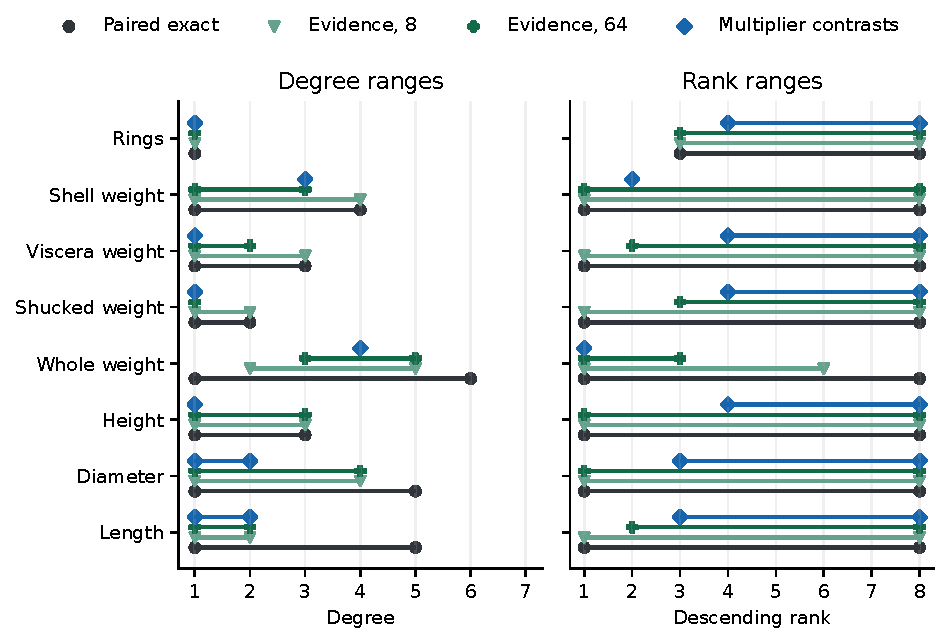
\includegraphics[width=\textwidth]{Fig_cross_section.pdf}
\caption{All eight Abalone degree and rank ranges after identical path projection. P, E8 and E64 have finite-sample guarantees under the stated IID model; M-C has asymptotic multiplier calibration. Population degree ties retain their full rank ranges.}\label{fig:cross}\end{figure}

\subsection{Which conclusions change after projection?}\label{sec:decision-application}
The primary question is which measurements can be certified as leaves, excluded from hub status, or placed within the top three. These are statements about the marginal association tree; leaf status alone does not justify removing a measurement from a predictive model. Table~\ref{tab:decision-abalone} separates the gain from replacing one matching by E64 from the gain due to subsequent optimization.


\begin{table}[H]\centering\small
\setlength{\tabcolsep}{4pt}
\caption{Abalone pooled: concrete conclusions under the IID working model and a separately chosen calibration. All rows use local edge comparisons. Fixed and excluded denote counts among eight measurements. The last two columns concern whole weight. P is one-matching exact McNemar--Holm.}\label{tab:decision-abalone}
\begin{lrbox}{\resultsbox}\begin{tabular}{llrrrr}
\toprule
Test & Projection & Fixed & Excluded & Degree & Rank\\
\midrule
P & Full LP & 1 & 1 & [1,6] & [1,8]\\
E64 & Minor & 1 & 2 & [2,5] & [1,6]\\
E64 & Degree LP & 2 & 4 & [3,5] & [1,3]\\
E64 & Full LP & 2 & 4 & [3,5] & [1,3]\\
\bottomrule\end{tabular}\end{lrbox}\ifdim\wd\resultsbox>\linewidth\resizebox{\linewidth}{!}{\usebox{\resultsbox}}\else\usebox{\resultsbox}\fi\end{table}


With E64 fixed, the minor stage excludes length and shucked weight from hub status. Degree-only path projection additionally excludes viscera weight and ring count, certifies ring count as a leaf, and raises the lower degree of whole weight from two to three. Together with degree conservation, these statements place whole weight within the top three. It is certified to have strictly greater degree than length, shucked weight, viscera weight and ring count in every population-optimal tree. The extra 56 ordered-pair LP objectives change none of the reported degree or rank endpoints. The top-three statement has a simple structural explanation. The eight degrees sum to 14. If whole weight and three competitors each had degree at least three, these four vertices plus the four remaining positive degrees would sum to at least 16. At most two competitors can therefore match or exceed whole weight. The inferential conclusion is four excluded hubs and a top-three restriction, with the identity of a unique population hub still unresolved.

Table~\ref{tab:decision-populations} reports the entire E64 local-family measurement grid, including cases with no new decision. At $n=1307$ and $1528$, degree LP certifies ring count as a leaf in the female and male Abalone strata, respectively; neither minor projection resolves those degrees. In the infant stratum, shucked weight is already a certified leaf before LP. The corresponding guarantees require an IID model separately within each analysed population. The comparisons across populations, methods and families are descriptive and have no joint 95\% coverage statement.


\begin{table}[H]\centering\small
\setlength{\tabcolsep}{4pt}
\caption{All 12 measurement populations: E64 local-family decision counts, minor $\to$ degree-only LP. Full ordered-pair projection gives the same rank endpoints as degree-only LP in every row. Dry Bean remains a computational stress study because the sampling design and repeated rows limit a population interpretation.}\label{tab:decision-populations}
\begin{lrbox}{\resultsbox}\begin{tabular}{lrrrrr}
\toprule
Population & $n$ & $p$ & Fixed & Excluded & Top three\\
\midrule
Abalone pooled & 4177 & 8 & 1 $\to$ 2 & 2 $\to$ 4 & 0 $\to$ 1\\
Abalone F & 1307 & 8 & 0 $\to$ 1 & 0 $\to$ 1 & 0 $\to$ 0\\
Abalone I & 1342 & 8 & 1 $\to$ 1 & 1 $\to$ 1 & 0 $\to$ 0\\
Abalone M & 1528 & 8 & 0 $\to$ 1 & 0 $\to$ 1 & 0 $\to$ 0\\
Bean Barbunya & 1322 & 16 & 0 $\to$ 0 & 0 $\to$ 0 & 0 $\to$ 0\\
Bean Bombay & 522 & 16 & 0 $\to$ 0 & 0 $\to$ 0 & 0 $\to$ 0\\
Bean Cali & 1630 & 16 & 0 $\to$ 0 & 0 $\to$ 0 & 0 $\to$ 0\\
Bean Dermason & 3546 & 16 & 0 $\to$ 0 & 0 $\to$ 0 & 0 $\to$ 0\\
Bean Horoz & 1928 & 16 & 0 $\to$ 0 & 0 $\to$ 0 & 0 $\to$ 0\\
Bean Seker & 2027 & 16 & 0 $\to$ 0 & 0 $\to$ 0 & 0 $\to$ 0\\
Bean Sira & 2636 & 16 & 0 $\to$ 0 & 0 $\to$ 0 & 0 $\to$ 0\\
Bean Pooled & 13611 & 16 & 0 $\to$ 0 & 0 $\to$ 0 & 0 $\to$ 0\\
\bottomrule\end{tabular}\end{lrbox}\ifdim\wd\resultsbox>\linewidth\resizebox{\linewidth}{!}{\usebox{\resultsbox}}\else\usebox{\resultsbox}\fi\end{table}


Across all 192 original method--family--population analyses, degree-only LP adds at least one of the stated decisions in 32 analyses. Full pair projection gives exactly the same rank endpoints in 188 of 192 analyses. Its remaining benefit is six additional hub exclusions across four analyses: female Abalone with multiplier rectangles and male Abalone with P, each under both comparison families. These four analyses concern two populations and are not independent confirmations. No stage produces a new unique-hub declaration on the measurement grid. Dry Bean's E64 degree widths narrow, but no leaf, hub exclusion or top-three restriction is certified, even in the pooled sample of 13,611 records. This distinguishes a narrower numerical bound from a new substantive conclusion.


\section{Computation matched to the inferential question}\label{sec:cost}
The decision-first workflow uses a fixed calibration and comparison family, then adds optimization only for the desired output. We benchmark one-matching P and E64 on all 12 measurement populations and the first replication of each of the 13 $p=12$ simulation cells with $n\ge1008$: 50 cases in total. This sample rule is independent of benchmark outcomes. Each case and stage runs in a fresh process, with one untimed warm-up and three timed repetitions, serial execution, one pinned CPU, and one BLAS/OpenMP/HiGHS thread. Interpreter startup and data loading are excluded. Projection timings include the minor construction, LP work and independent rational-certificate checks. Calibration is timed separately, including full Kendall computation for E64. These are computational repetitions of fixed instances, not Monte Carlo estimates of inferential power.
The recorded environment is Python 3.12.14, NumPy 2.3.5 and SciPy 1.17.0 on an AMD EPYC 9V74 80-Core Processor processor. Raw per-run timings, process peak resident memory, CPU affinity and all reconstructed endpoints are archived. Peak resident memory includes imports, input and warm-up; it is not interpreted as incremental solver storage.


\begin{table}[H]\centering\small
\setlength{\tabcolsep}{4pt}
\caption{Controlled cost for E64 on pooled Abalone ($p=8,n=4177$). Seconds are medians of three timed repetitions. Each projection time includes the minor stage; calibration is separate. Degree-only and full LP have identical degree and rank endpoints.}\label{tab:cost-abalone}
\begin{lrbox}{\resultsbox}\begin{tabular}{lrr}
\toprule
Stage & LP objectives & Seconds\\
\midrule
Edge calibration & -- & 0.1400\\
Minor & 0 & 0.0013\\
Degree LP & 16 & 0.0391\\
Full LP & 72 & 0.1534\\
\bottomrule\end{tabular}\end{lrbox}\ifdim\wd\resultsbox>\linewidth\resizebox{\linewidth}{!}{\usebox{\resultsbox}}\else\usebox{\resultsbox}\fi\end{table}


For this example, degree-only projection requires 16 instead of 72 LP solves and takes 0.0391 rather than 0.1534 seconds, a 74.5\% reduction in projection time. E64 calibration itself takes 0.1400 seconds, so the 3.92-fold projection speedup is not an end-to-end speedup of the entire statistical method.


\begin{table}[H]\centering\small
\setlength{\tabcolsep}{4pt}
\caption{All 50 benchmark cases, by data source and dimension. Each entry is the median across case-specific medians of three runs. Empty order relations and forced unique trees skip redundant LP solves, including in the simulated group. These medians therefore reflect the stated case mix as well as dimension.}\label{tab:cost-grid}
\begin{lrbox}{\resultsbox}\begin{tabular}{lrrrrr}
\toprule
Source & $p$ & Cases & Minor (s) & Degree LP (s) & Full LP (s)\\
\midrule
Abalone & 8 & 8 & 0.0018 & 0.0415 & 0.1561\\
Simulated & 12 & 26 & 0.0033 & 0.0755 & 0.3904\\
Dry Bean & 16 & 16 & 0.0078 & 0.1701 & 1.1497\\
\bottomrule\end{tabular}\end{lrbox}\ifdim\wd\resultsbox>\linewidth\resizebox{\linewidth}{!}{\usebox{\resultsbox}}\else\usebox{\resultsbox}\fi\end{table}


The degree-only stage is the economical default for degree bounds and the tested partial decisions. Ordered-pair objectives remain an optional refinement when an unresolved comparison or rank question warrants the extra work. Their benefit should be reported as a changed conclusion, along with cost, rather than inferred from the number of solved programs. The audit is retrospective and the measured costs are instance- and hardware-specific; it establishes the gains on this complete evaluation grid rather than universal dominance of a projection stage.

